\section{Problèmes rencontrés, problèmes résolus}

Le développement de GuitarTutor ne s'est pas fait sans heurts. Nous sommes néanmoins parvenus à résoudre les différents problèmes auxquels nous avons été confrontés au cours des phases de développement.

\subsection{Reprise de code}

Comme c'était prévu, la reprise du code existant fut notre première grande étape de développement. Passé le moment de découragement lié à l'absence total de commentaires et de documentation dans la grande majorité du code source qui nous intéressait, nous nous sommes attelés à ``débroussailler'' le dépôt en mettant en place une documentation, en commentant le code, ainsi qu'en supprimant purement et simplement les portions inutilisées, qui représentaient tout de même une portion loin d'être négligeable (parfois de simples fonctions, parfois des fichiers, et parfois des dossiers entiers\dots).

Par ailleurs, du fait que le projet ait été constitué de plusieurs blocs de code émanant de différentes équipes de développeurs, nous avons pu remarquer que les conventions de codage n'avaient pas été harmonisées. Nous avons pris soin de réparer cette erreur afin de faciliter la relecture et donc la réutilisation de ce même code.

Passés ces quelques semaines de nettoyage et d'assimilation du code existant, nous avons pu commencer à apporter les modifications établies dans le cahier des charges, bien que, tout au long du développement, nous ayons continué la refactorisation (par exemple les suppressions de certaines bibliothèques, évoquées plus loin dans ce rapport).

\subsection{Refonte de l'interface du lecteur}

La refonte totale de l'interface du lecteur s'est présentée comme un véritable challenge. Il s'agissait en effet de supprimer tout ce qui concernait l'interface dans le projet existant, et d'y mettre à la place notre propre code. Évidemment, il n'était pas question de se limiter à une structure identique à l'interface existante, celle-ci étant véritablement limitée en terme de fonctionnalités, et m\^eme carrément repoussante pour un jeune guitariste débutant. Fort heureusement, le lecteur était déjà plut\^ot bien décomposé selon le modèle MVC, ce qui nous a tout de m\^eme motivé à tenter l'expérience.

La nouvelle interface a donc été développée seule, totalement séparée du reste du projet, en utilisant des faussaires pour simuler une grille d'accords, et selon une maquette que nous avions soumise à nos clients (voir figure \ref{annexe_proto_player} en annexe). Ce n'est qu'au bout de plusieurs semaines de développement que nous avons enfin pu intégrer la nouvelle interface au reste du projet. Cette intégration ne s'est pas faite sans heurts, mais a finalement aboutie, comme nous l'espérions (voir figure \ref{interface_player}).

\begin{figure}[H]
\begin{center}
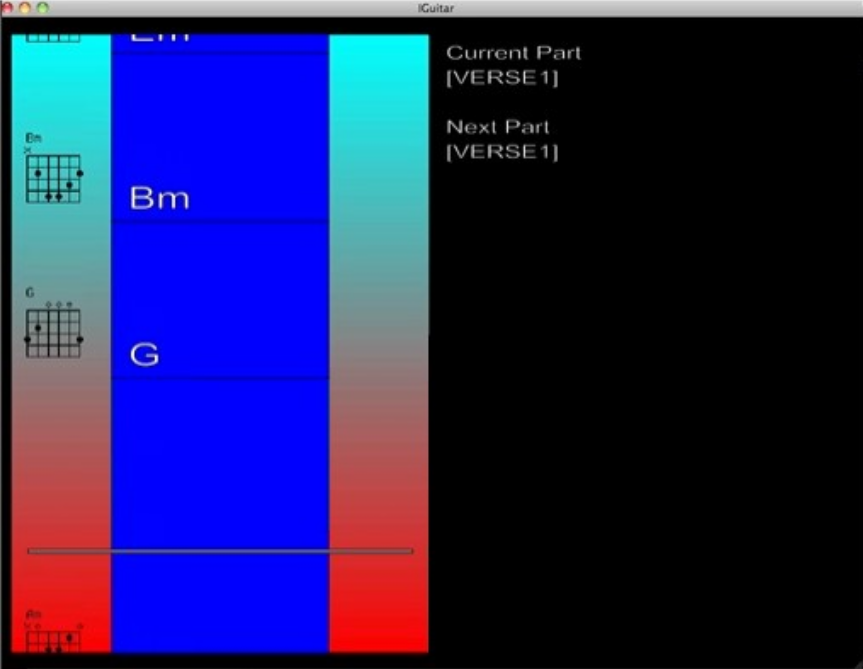
\includegraphics[width=175px]{ancien_player.png}
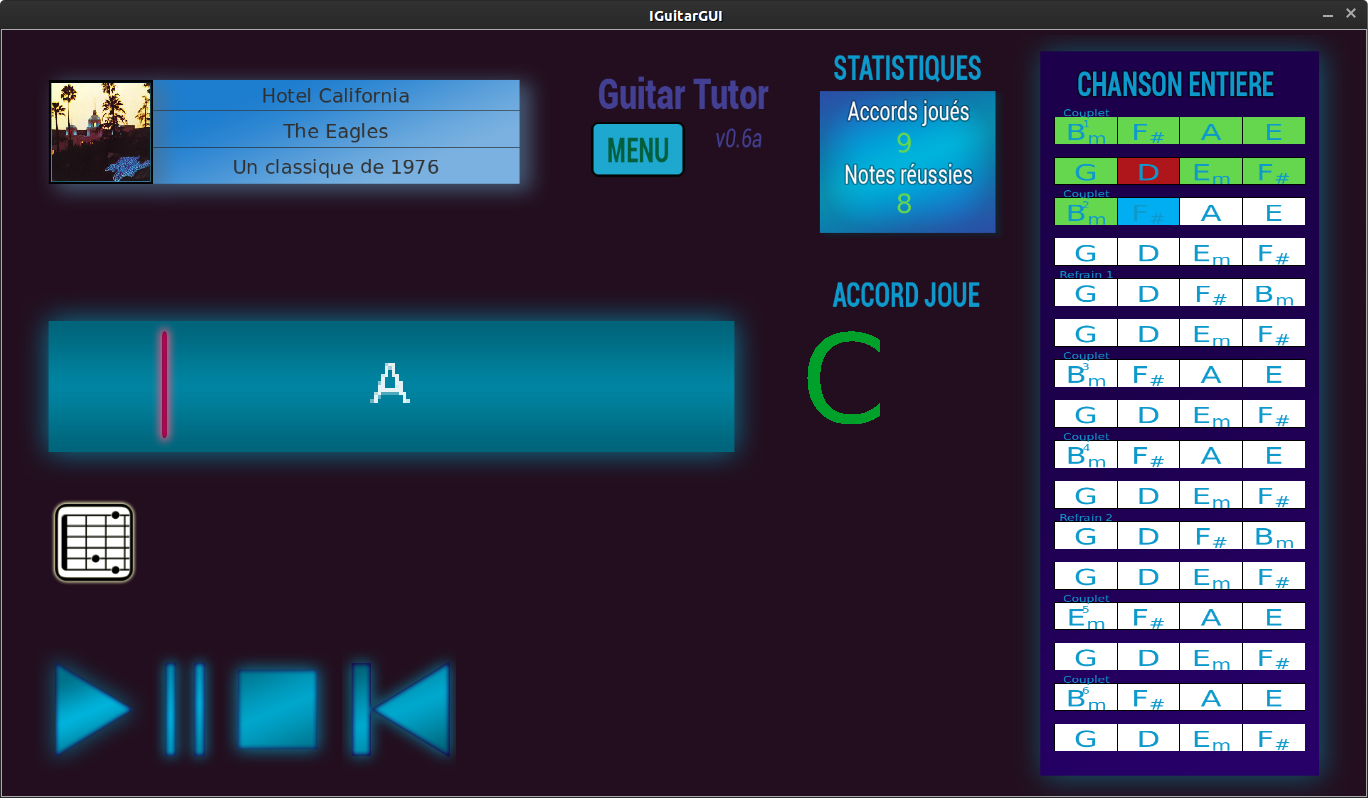
\includegraphics[width=275px]{interface_player.png}
\caption{L'interface du lecteur a été entièrement refaite}
\label{interface_player}
\end{center}
\end{figure}

\subsection{Portabilité}

La portabilité du logiciel, notamment sur Mac OS et Windows, faisait partie des principales demandes des clients. Les librairies utilisées jusque là était censées fonctionner à la fois sur Mac OS, Windows et GNU/Linux, et c'était une bonne raison pour ne pas en changer.

Nous nous sommes cependant rapidement rendus à l'évidence: on ne développe pas un logiciel portable simplement en utilisant des librairies portables.

\subsubsection*{Sur Mac OS}

Personne, dans notre équipe, n'ayant une machine sous Mac OS, nous avons dû nous contenter d'une version de Mountain Lion en machine virtuelle. Outre un problème d'extrême lenteur lors de la compilation et divers autres soucis liés à la connexion internet et la reconnaissance des ports USB, il était impossible de vérifier le bon fonctionnement du lecteur, puisque l'entrée audio de la VM n'était pas activée. Nous avons donc pendant longtemps développé \textit{``à l'aveugle''} sous Mac OS, où tout ce que nous pouvions faire était de vérifier que la compilation se faisait correctement.

Fort heureusement, un test sur une vraie machine Mac début mars nous a confirmé que le projet était bien compatible, et nous en avons également profité pour vérifier le fonctionnement de notre installateur.

\subsubsection*{Sur Windows}

Le portage sous Windows a été périlleux, car le système de base n'a rien à voir avec les systèmes ayant pour base Unix et respectant
les normes POSIX que sont Linux et Mac OS X.

Notre premier réflexe a été d'utiliser MinGW qui est livré par défaut avec Qt. Néanmoins, un problème
dans la librairie winpthreads qui était livré avec la version de MinGW qui était elle-même livrée avec Qt 4.8 nous a
forcé à passer sur la librairie BOOST C++ pour un temps. De plus, en raison de l'utilisation de certaines fonctionnalitées modernes
de GCC 4.7 sous Linux, qui n'étaient pas disponibles sous MinGW 4.2, la compilation ne marchait pas sous Windows.

Nous effectuions donc un cross-compiling sous Linux, ce qui représentait une certaine perte de temps pour les tests.

Il a de plus fallu recompiler libsndfile qui n'était pas disponible directement sous Windows.

\paragraph{Arrivée de Qt5}
De ce point de vue, l'arrivée de Qt 5 a été salvatrice pour notre projet : en effet, elle mettait à jour MinGW
avec la dernière version de gcc, ce qui a permis une compilation directe depuis Windows, ainsi que la suppression des
threads BOOST pour un retour aux pthreads.

Nous avons de plus travaillé sur une branche qui permette la compilation avec MSVC, le compilateur C++ Microsoft.

Néanmoins, ce compilateur ne supporte pas le standard C99, qui est utilisé dans la librairie EHPCP pour représenter les types complexes.

Nous avons donc fait une tentative de portage en utilisant la classe C++ Complex, mais les performances étaient moindres au final,
ce qui nous a poussé à rester sous MinGW.

\paragraph{Installation}
Une des autres particularités de Windows est qu'il n'y a pas de système de gestion de paquetage comme sous la majorité des systèmes Linux et Mac OS X.
Il est donc nécessaire de créer nous-même un installeur, nous avons pour ce faire utilisé Advance Installer dans sa version gratuite.

Ce logiciel permet un déploiement facile : création d'icônes dans le menu démarrer, sur le bureau, gestion des mises à jour...

\paragraph{Portaudio et performance audio basse-latence}
Contrairement à Linux et Mac OS X, dont les couches audio ALSA (pour Linux) et CoreAudio (pour Mac OS X) permettent immédiatement
des basses latences, ce n'est pas le cas sous Windows.

Cela pose problème pour le jeu de guitare : en effet, la latence de base du mixeur Windows est d'environ 40 millisecondes.
Et des mesures ont montré que l'oreille humaine arrivait à percevoir un décalage à partir de 10 millisecondes, et que cela devenait gênant pour le jeu à partir de 20 millisecondes.

Une solution a été développée par Steinberg (l'éditeur du séquenceur Cubase) : le protocole ASIO.

Ce protocole permet d'atteindre de très basses latences (parfois jusqu'à moins d'une milliseconde) avec
du matériel professionnel et de basses latences avec ASIO4ALL, un logiciel qui permet d'utiliser des cartes son standard de PC avec le protocole ASIO.

Le problème pour l'incorporation de cette technologie dans le projet est qu'il est nécessaire de compiler PortAudio avec le SDK ASIO, ce qui
ne peut se faire qu'avec MSVC, le compilateur Microsoft.
Comme l'algorithme de name-mangling de MSVC est incompatible avec celui de MinGW / GCC, il est nécessaire de recompiler tout le projet avec MSVC, ce qui cause la perte de performance vue plus haut.
De plus, il faut remplacer la DLL portaudio fournie dans le livrable avec la DLL compilée avec le support ASIO, ce qui fait
que le logiciel ne pourra pas s'exécuter sur un ordinateur sans ASIO4ALL ou une carte son professionnelle fournissant un pilote ASIO.


\subsubsection*{Sur GNU/Linux}

Il s'agit du seul des trois systèmes d'exploitation pour lequel nous n'avons pas eu de problème particulier, mais aussi le seul qui n'était pas demandé. Peut-être est-ce simplement parce que nous avons tous commencé à coder directement sur celui-ci.
